\documentclass[12pt]{exam}

\usepackage{setspace}
\usepackage{listings}
\usepackage{graphicx,subfigure,wrapfig}
\usepackage{multirow}
\usepackage[colorlinks=true,urlcolor=blue]{hyperref}
\usepackage[margin=20mm]{geometry}
\usepackage{xepersian}
\usepackage{fontspec}
\settextfont[ExternalLocation]{XB Niloofar.ttf}
   
\newcommand{\class}{طراحی پایگاه داده‌ها}
\newcommand{\term}{نیم‌سال دوم 02-03}
\newcommand{\college}{دانشکده مهندسی کامپیوتر}
\newcommand{\prof}{استاد: مهدی آخی }

\singlespacing 
\parindent 0ex

\lstset{
keywordstyle=\textbf,
identifierstyle=, 
stringstyle=\ttfamily,
commentstyle=\color{LimeGreen}, 
stringstyle=\ttfamily,
numberstyle=\footnotesize,
showstringspaces=false} 
\begin{document}


% -------------------------------------------------------
%  Thesis Information
% -------------------------------------------------------

\newcommand{\ThesisType}
{سمینار}  % پایان‌نامه / رساله
\newcommand{\ThesisDegree}
{کارشناسی ارشد گرایش معماری کامپیوتر}  % کارشناسی / کارشناسی ارشد / دکتری
\newcommand{\ThesisMajor}
{مهندسی کامپیوتر}  % مهندسی کامپیوتر
\newcommand{\ThesisTitle}
{پروژه درس طراحی پایگاه ‌داده‌ها}
\newcommand{\ThesisAuthor}
{ملیکا علیزاده - ثمین اکبری - معین آعلی}
\newcommand{\ThesisSupervisor}
{مهدی آخی}
\newcommand{\ThesisDate}
{نیم‌سال دوم 02-03}
\newcommand{\ThesisDepartment}
{دانشکده مهندسی کامپیوتر}
\newcommand{\ThesisUniversity}
{دانشگاه صنعتی شریف}

% -------------------------------------------------------
%  English Information
% -------------------------------------------------------

\newcommand{\EnglishThesisTitle}{Database-Design Course Project}


\pagestyle{empty}

\begin{center}


\includegraphics[scale=0.2]{logo.png}

\vspace{0.5cm}
\ThesisUniversity \\[-0.3em]
\vspace{0.5cm}
\ThesisDepartment\\

\begin{large}
\vspace{0.5cm}


%\ThesisMajor

\end{large}

\vspace{1.5cm}

{عنوان:}\\[1.2em]
{\LARGE\textbf{\ThesisTitle}}\\ 
\vspace{1cm}
\begin{latin}
{\Large\textbf\EnglishThesisTitle}
\end{latin}

\vspace{2cm}

{نگارش}\\[.5em]
{\large\textbf{\ThesisAuthor}}

\vspace{1.5cm}

{استاد}\\[.5em]
{\large\textbf{\ThesisSupervisor}}

\vspace{1cm}



\vspace{2cm}

\ThesisDate

\end{center}

\newpage


% These commands set up the running header on the top of the exam pages
\pagestyle{head}
\firstpageheader{}{}{}
\runningheader{صفحه \thepage\ از \numpages}{ملیکا علیزاده - ثمین اکبری - معین آعلی}{\class}
\runningheadrule

\pagebreak

\subsection*{\underline{تقسیم‌بندی پروژه}}
\subsubsection*{تسک‌های مربوط به عضو اول: \href{https://github.com/MelikaAlizadeh}{ملیکا علیزاده}}
\begin{enumerate}
	
	
	\item شناسایی موجودیت ها (Entities) از پروژه
	
	\item شناسایی صفات (Attributes) از پروژه
	
	\item طراحی موجودیت ها و صفات در Draw.io
	
	\item طراحی روابط در Draw.io
	
	\item نوشتن توضیحات برای ERD
	
\end{enumerate}
\subsubsection*{تسک‌های مربوط به عضو دوم: \href{https://github.com/saminakbari}{ثمین اکبری} }
\begin{enumerate}
	
	\item شناسایی موجودیت ها (Entities) از پروژه
	
	\item شناسایی صفات (Attributes) از پروژه
	
	\item طراحی موجودیت ها و صفات در Draw.io
	
	\item طراحی روابط در Draw.io
	
	\item نوشتن جبر رابطه‌ای
	
	
\end{enumerate}
\subsubsection*{تسک‌های مربوط به عضو سوم: \href{https://github.com/MoeeinAali}{معین آعلی}}
\begin{enumerate}
	
	\item ایجاد مخزن گیت هاب و تعریف مساله
	
	\item طراحی موجودیت ها و صفات در Draw.io
	
	\item آماده سازی لاتک (LaTeX) برای پاسخ های پروژه
	
	\item نوشتن جبر رابطه‌ای
	
	\item نوشتن جبر رابطه‌ای با LaTeX
	
	
\end{enumerate}

جزئیات تقسیم‌بندی کارها داخل این 
\href{https://github.com/MoeeinAali/DB-Project/issues/1}{Issue Github}
موجود است.

\pagebreak
\subsection*{\underline{نمودار رابطه-موجودیت}}

$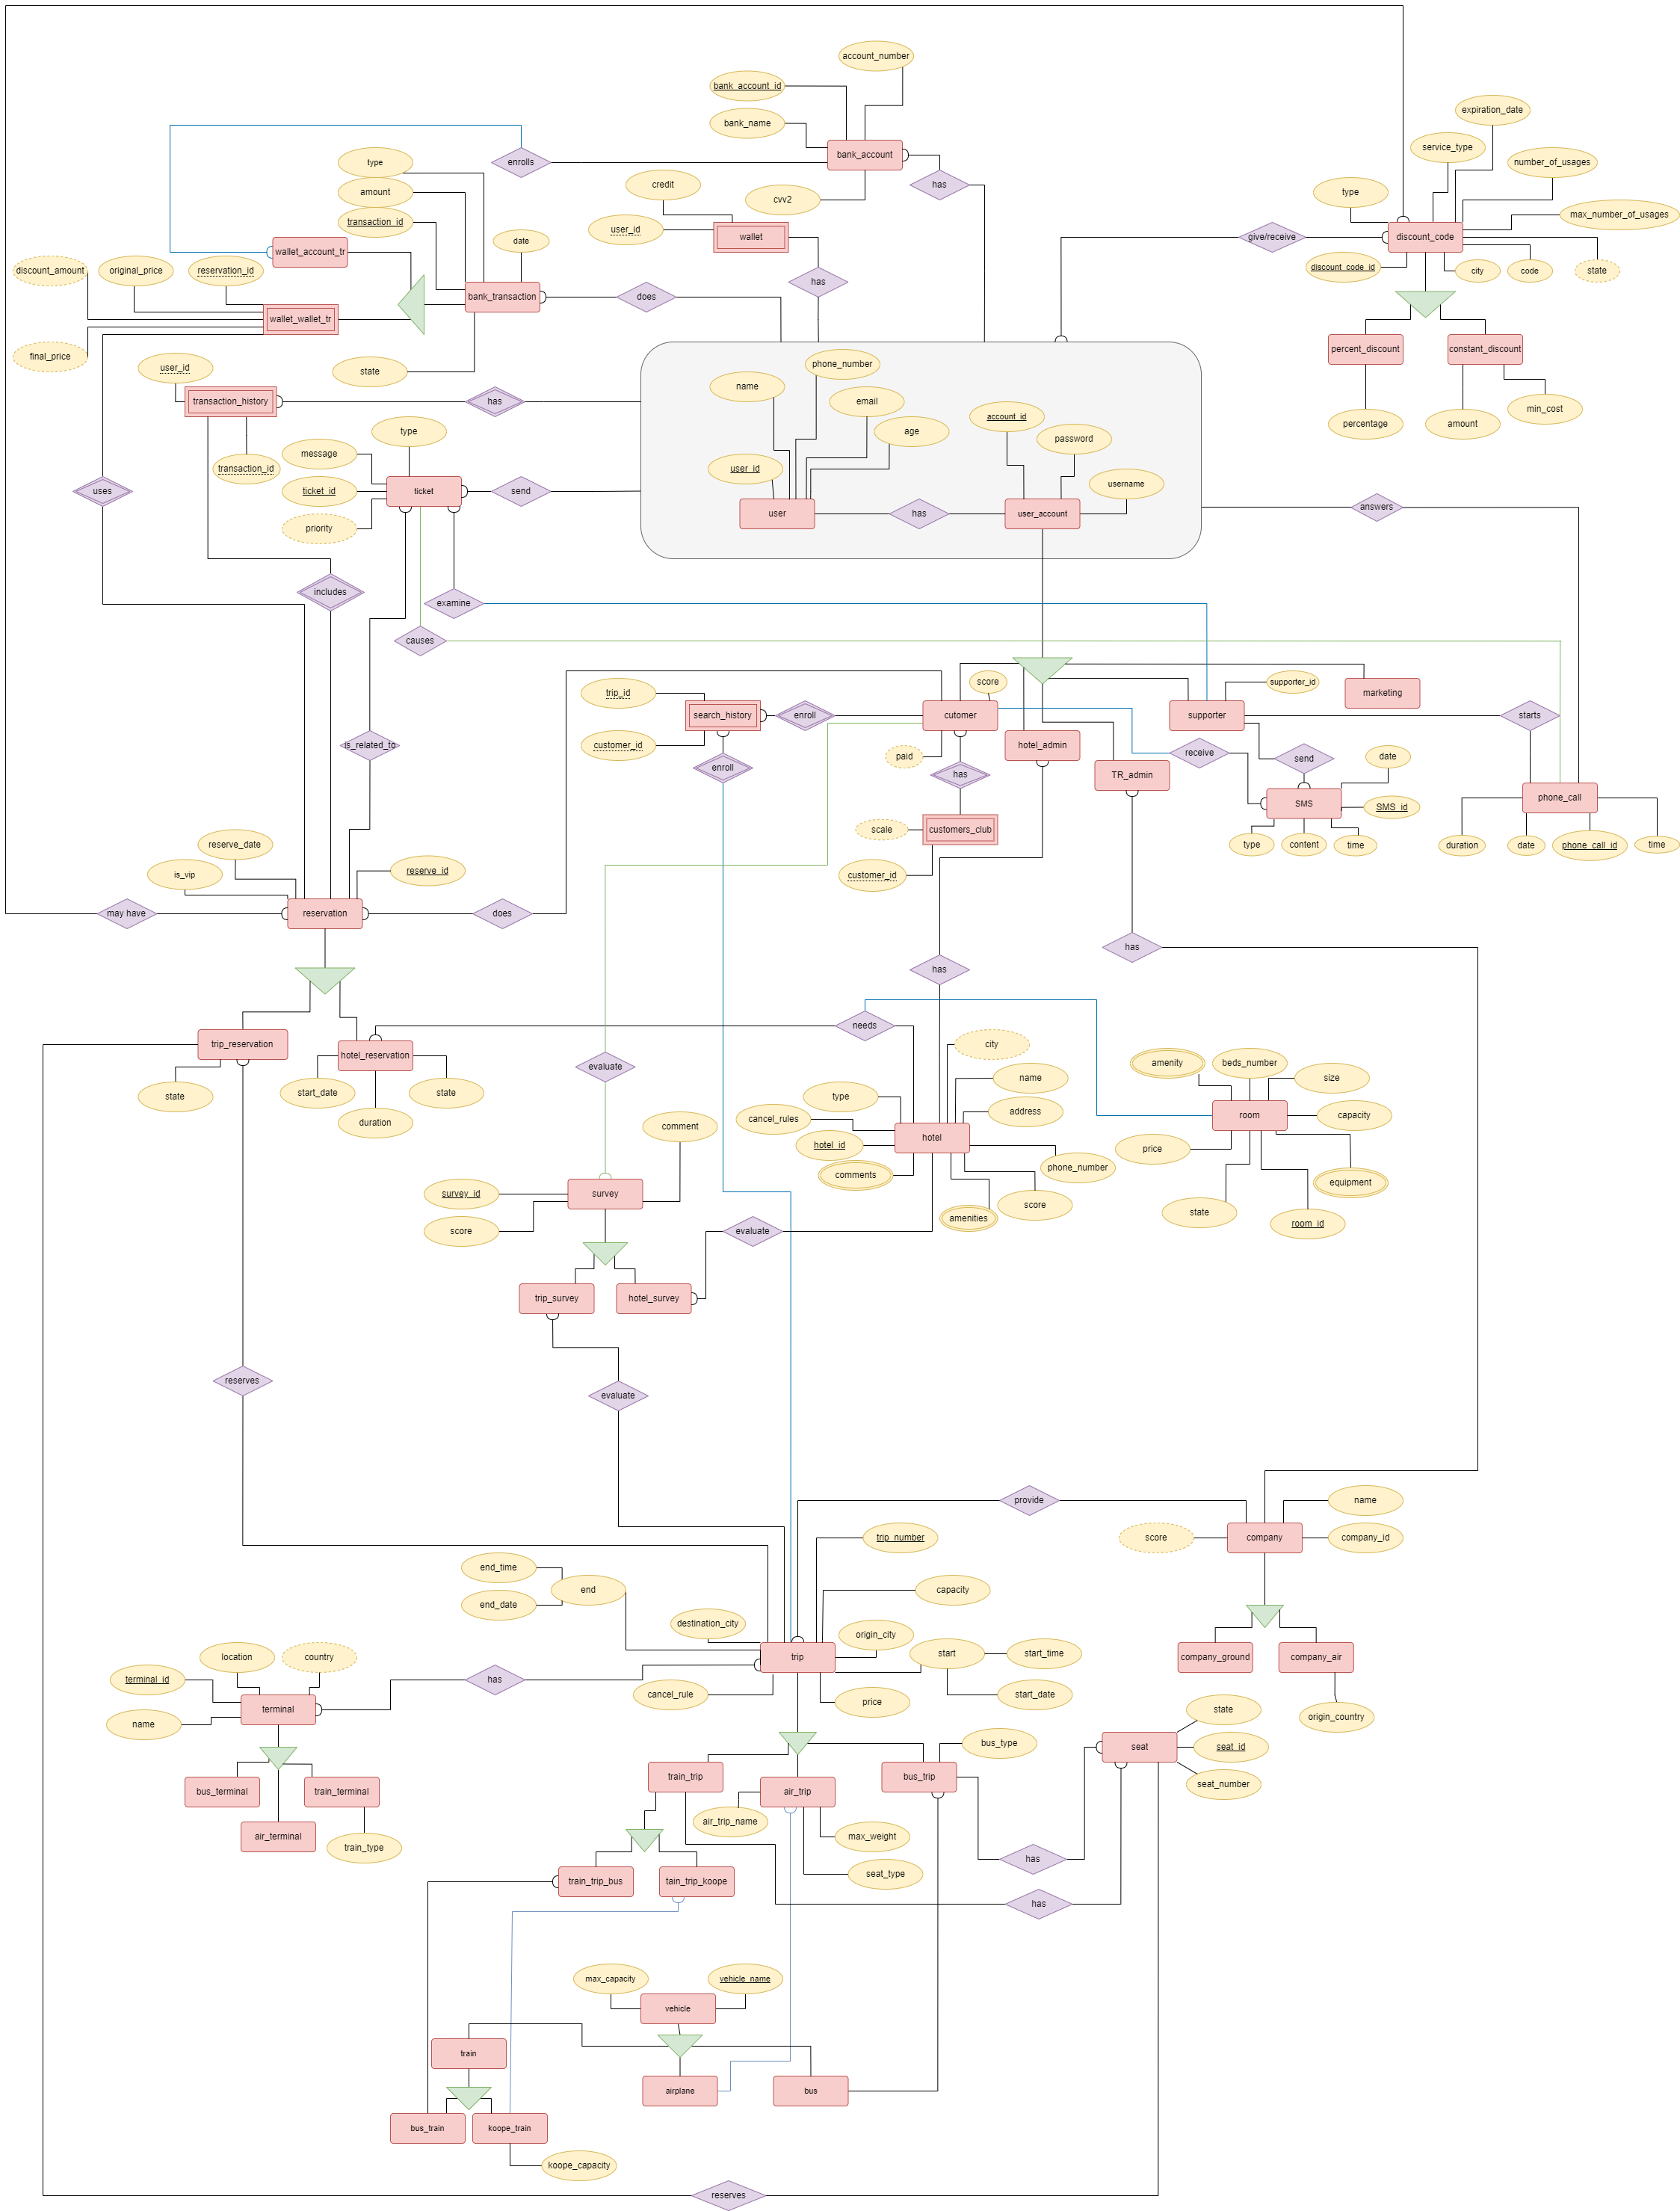
\includegraphics[width=1\linewidth]{figs/1.png}$

فایل Draw.io مربوط به ERD پروژه، داخل پیوست قرار دارد. 

در این بخش توضیحات مربوط به روابط مختلف این ERD آورده شده است:

\begin{itemize}
	\item مورد
	
توضیحات
	\item مورد 

توضیحات
	\item مورد 

توضیحات
\end{itemize}
\pagebreak

\subsection*{\underline{جبر رابطه‌ای}}

در این بخش پاسخ پرسمان‌های زیر با استفاده از جبر رابطه‌ای آورده شده است:

\begin{enumerate}
	\item
‌هواپیماهایی که در ۲۹ اسفند از تهران به مشهد می‌روند و بیشتر از ۵ صندلی خالی دارند را پیدا کنید.




	\item
هتل‌هایی که در تاریخ ۱ فروردین اتاق دو تخته‌ی خالی دارند و امکانات استخر و باشگاه و \linebreak امتیاز بالای ۴ دارند را پیدا کنید.




	\item
	 میزان تخفیفی که مشتریان با استفاده از کد تخفیف  norouz  دریافت کرده‌اند را حساب کنید.
	 
	 
	 
	 
	\item
	 تماس‌های پشتیبانی که در مورد هتل الماس بوده‌اند را پیداکنید.
	 
	 
	 
	 
	 
	\item
مجموع هزینه‌هایی که‌ به واسطه باشگاه مشتریان در ماه فروردین کسر شده‌است را بیابید.




	\item
تعداد رزروهایی که در مدت معین پرداخت نشده، و لغو شده‌اند را بیابید.





	\item
تعداد مسافرین به تفکیک نوع سفر(قطار، اتوبوس، هواپیما) در تعطیلات نوروز(اول تا 13 فروردین ماه) را بیابید.





	
	\item
	 آمار تعداد کنسلی رزروهای هتل‌ها در 5 شهر با بیشترین خرید بلیط به مقصد آنجا به‌ تفکیک ستاره هتل‌ها را بیابید.
	 
	 
	 
	 
	
	\item
	 همه مسافرانی که در پرواز $W1296$ در تاریخ 6 فروردین برای همان روز در هتلی با بیشترین اتاق خالی رزرو دارند.
	
	
	
	
	
	\item
	 مشتریانی را بیابید که برای تاریخ ۱ فروردین، بلیط به مقصد شهر بابلسر رزرو کرده‌اند و همچنین \linebreak با کد تخفیف ۳۰ هزار تومانی (که در بخش CRM به‌ آن اشاره شد) رزرو هتل خود را هم از سایت انجام داده‌اند.
	 
	 
	 
	 
	
\end{enumerate}

\end{document}